% Poster based on beamerposter.  For more information, see:
% http://www-i6.informatik.rwth-aachen.de/~dreuw/latexbeamerposter.php

\documentclass[final,svgnames,dvipsnames,table]{beamer}
\mode<presentation>{
  \usetheme{HongKong}
}
\usepackage[orientation=portrait,size=a0,scale=1.2]{beamerposter}
%\usepackage[french]{babel}   % "babel.sty" + "french.sty"
\graphicspath{{./}{../figs/}}
\usepackage[utf8]{inputenc}
\usepackage{multicol}
\usepackage{subfigure}
\usepackage{caption}
%\usepackage{subcaption}


%\usepackage{eurosym}
\usepackage{MnSymbol}
\usepackage{tikz}
\usetikzlibrary{arrows,shapes, calc}
\usepackage{xcolor}
\usepackage{array}
\usepackage{hyperref}
\usepackage{cleveref}
%% \usepackage[natbib=true, bibstyle=authoryear, maxnames=2,
%%   citestyle=authoryear-comp]{biblatex}
%% \bibliography{huynh.2016.icpr}
\usepackage{amsmath,,amssymb,amsfonts}
\usepackage{stmaryrd}
\usepackage{tabularx}

\usepackage{relsize}
\usepackage{setspace}

\usepackage{pifont}% http://ctan.org/pkg/pifont
\newcommand{\cmark}{\ding{51}}%
\newcommand{\xmark}{\ding{55}}%

\usepackage{multirow, multicol}
%\usepackage[usenames,dvipsnames,svgnames,table]{xcolor}


%\newcommand{\etal}{{\it et al.}\xspace}

%\usepackage[numbers,sectionbib]{natbib}

% Specific definitions
\definecolor{bglayer}{named}{ta3aluminium}

%\setbeamercolor{block body}{fg=red}
%\setbeamercolor{block itemize item example}{fg=red}
%\setbeamercolor*{block title example}{fg=red}
%\AtBeginEnvironment{exampleblock}{\setbeamercolor{itemize item subitem}{fg=red}}
%\setbeamercolor{local structure itemize item}{fg=red}

\usepackage{xspace}

\newcommand{\Lab}{{\ensuremath{L a^{*} b^{*}}}\xspace}


\title{%\fontsize{64}{60}\selectfont
  \vskip36pt Spherical fluorescent particle segmentation and tracking in 3D confocal microscopy \\[16pt]
  %\texorpdfstring{\colorbox{yellow}{\color{red}{~A Mathematical Morphology Approach~}}}{ } 
  }
\author{\'{E}lodie Puybareau\inst{1,2} \and Edwin Carlinet\inst{1} \and Alessandro Benfenati\inst{2} \and Hugues Talbot\inst{2,3} \\}

\institute{
EPITA Research and Development,
14-16 rue Voltaire, F-94276 Le Kremlin-Bicetre
\and
Université Paris-Est, ESIEE Paris, 2 boulevard Blaise-Pascal, F-93162 Noisy-le-Grand
\and
CentraleSupelec, Centre de Vision Numérique, INRIA équipe OPIS, 3 rue Joliot-Curie, F-91190
Gif-sur-Yvette.\\
\ \\
}

\date{ISMM 2019 ---  Saarbr\"ucken --- July 8-10, 2019}

\logoleft{%
  \vspace{0.5cm}

\hspace*{-2.5cm}
\includegraphics[width=5cm]{lrde.png} \\
\hspace*{-2.5cm}
\includegraphics[width=5cm]{epita-logo} \\
\hspace*{-2.5cm}
\includegraphics[width=10cm]{logo-CentraleSupelec.png}\\
\hspace*{-2.5cm}
\includegraphics[width=5cm]{UPS_Logo_Transparent.png}
}

\logoright{%
  \vspace*{1.5cm}
  
\includegraphics[width=5cm]{Logo_LIGM_Transparent.png} \\[15pt]
  
\includegraphics[width=5cm]{Logo_ESIEE_Transparent.png} \\
  
\includegraphics[width=7cm]{Logo_UPE_transparent.png} \\
  
\includegraphics[width=7cm]{Inria_Logo_Transparent.png}
}
\setbeamertemplate{footline}[text line]{\hfill{}\tiny ISMM 2019 ---
  Saarbr\"ucken, Germany --- July 8-10, 2019}

%\setbeamertemplate{background canvas}{%
%\tikz[remember picture,overlay]{\fill[color=blue] (-70, -70) ++(-1,0.5) rectangle ++(23.5,-26.5);
%  \fill[color=blue] (10, 70) ++(22.5, 0.5) rectangle ++(58,-70);}
%}

\definecolor{MyGray}{rgb}{0.1,0.3,0.4}



\begin{document}
\setbeamertemplate{caption}{\raggedright\insertcaption\par}
%% \usebackgroundtemplate{%
%%   \tikz[remember picture, overlay]{
%%     \coordinate [right=1] (midpoint) at (current page.west);
%%     %\filldraw[color=bglayer] (midpoint) ++(0.5, 14) rectangle ++(83,-21);
%%     %\filldraw[color=bglayer] (midpoint) ++(0.5, -27) rectangle ++(83,-22);
%%     %\filldraw[color=bglayer] (midpoint) ++(30, -27) rectangle
%%     %++(53.5,20);
%%     \filldraw[color=bglayer] (midpoint) ++(0.5, -69) rectangle ++(83,83);
%%     \fill[color=white] (current page.south west) rectangle ++(34.5,52);
%%   }
%% }



\begin{frame}[fragile]

%\vskip-1em
   \begin{exampleblock}{\bf At a glance}
    \centering

    \vskip .5em
    \begin{figure}
\centering
\subfigure[]{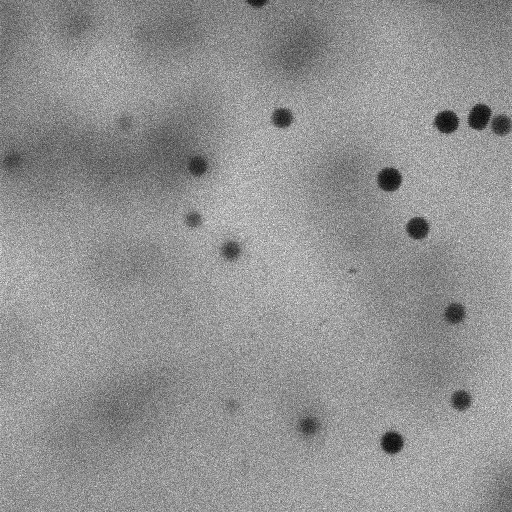
\includegraphics[width =  0.15\linewidth]{images/exp1_t01z5.png}}
\subfigure[]{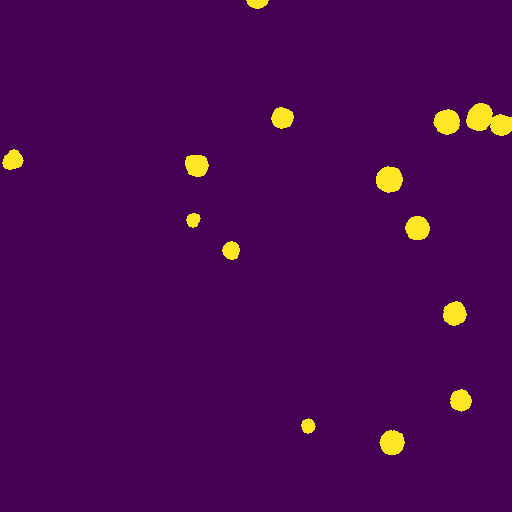
\includegraphics[width =  0.15\linewidth, clip, trim = 5cm 5cm 0cm 0cm]{images/orig_1.png}}
\subfigure[]{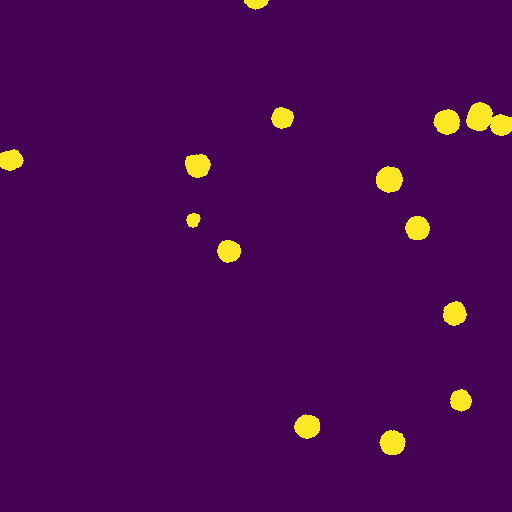
\includegraphics[width =  0.15\linewidth, clip, trim = 5cm 5cm 0cm 0cm]{images/orig_fermee_1.png}}
%\vspace{0.3em}
\subfigure[]{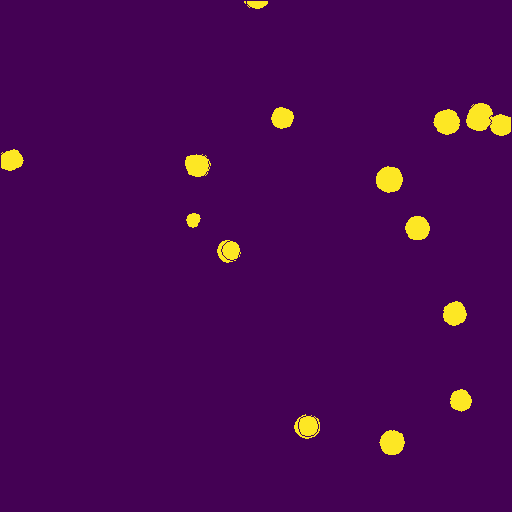
\includegraphics[width =  0.15\linewidth, clip, trim = 5cm 5cm 0cm 0cm]{images/orig_separ_1.png}}
\subfigure[]{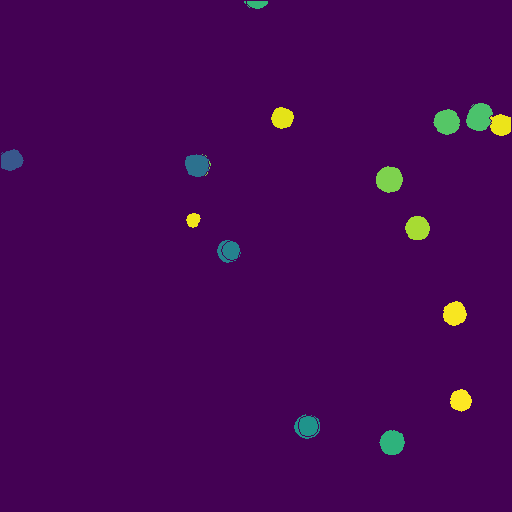
\includegraphics[width =  0.15\linewidth, clip, trim = 5cm 5cm 0cm 0cm]{images/toto.png}}
\caption{Results of the successive steps: (a) input image, and zoom on (b) initial segmentation, (c) 3D regularization, (d) bead separation, (e) individualization and labeling.}
\label{fig:temporal}
\end{figure}
    \begin{multicols}{2}
    \begin{description}
    \item[{\bf ~~Problem statement:}] ~ %
      \begin{itemize}
      \item Spherical fluorescent beads are used in many areas of
        physics and biology for positioning and tracking~{\color{cyan}\cite{benfenati2019efficient}};
      \item not many 3D segmentation methods exist for tracking in
        fluid: the particles move during acquisition due to Brownian
        motion~{\color{cyan}\cite{puybareau2017morphologicalposter}};
      \item radius distribution is known but not precise radius.
      \end{itemize} \bigskip %
      %
    \item[{\bf ~~Why our approach is interesting:}] ~ %
      \begin{itemize}
      \item segmentation and tracking are based on classical mathematical morphology operators;
      \item information is aggregated from 2D slices to find most likely
        position and radius;
      \item tracking and position estimation are achieved separately ;
      \item 0.1 subpixel accuracy is achieved in positioning.
      \end{itemize} \bigskip %
      %
    \item[{\bf ~~Key benefits:} ] ~ %
      \begin{itemize}
      \item our method works on beads with imprecisely known radii
      \item it can accurately segment, track and position 3D beads even
        in fluids
      \item can be used to measure Brownian diffusion coefficients
      \end{itemize}
    \end{description}
    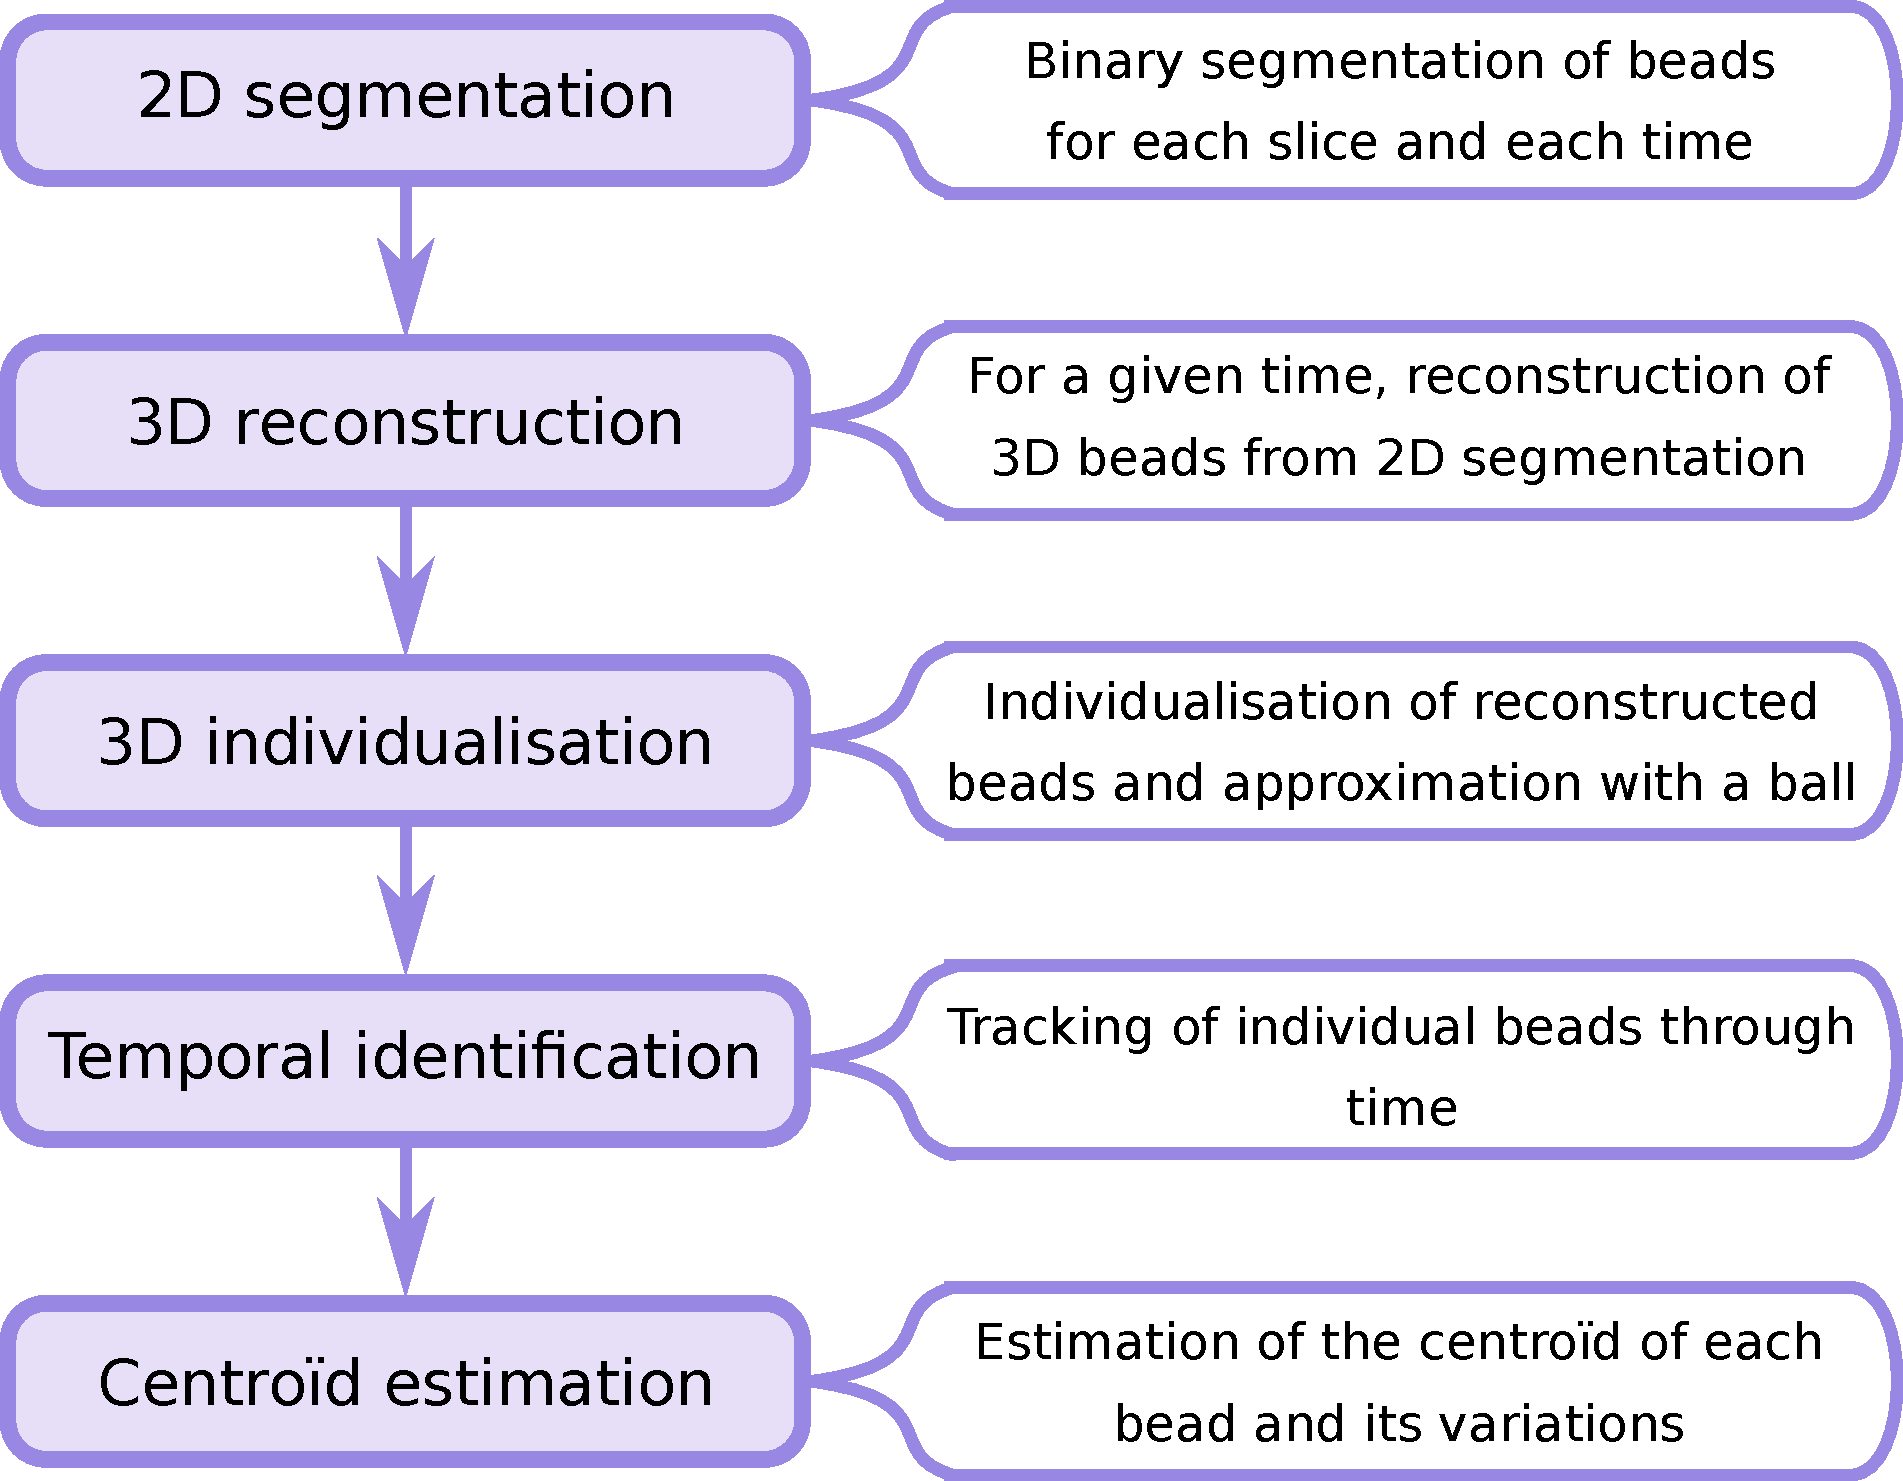
\includegraphics[width = 0.6\linewidth]{images/flowchart.pdf}
    \end{multicols}
   \end{exampleblock}
   
   
  \begin{columns}[t,totalwidth=\textwidth]
    %
    % LEFT
    %
    %\begin{column}{\textwidth}

   %\end{column}
   \begin{column}{0.32\textwidth}
   % ###############################################
   %\vskip .5em
    % ###############################################
    
    \begin{block}{\bf Segmentation and tracking}
      Segmentation and tracking consists of the following steps:
      \centering

      \vskip .5em
      \begin{itemize}
          \item 2D Segmentation pipeline: \\ \begin{enumerate}
\item Supression of small local minimas (closing by reconstruction with an initial dilation by a disk of radius 4).
\item Calculation of the min-tree of the previous result.
\item Filtering of nodes by combined criteria (size, grey-level intensity, contrast of component). 
\item Regularisation of the selected blobs.
\end{enumerate}
\vspace{2em}
\begin{figure}
\centering
\hspace{-3.3em}
\subfigure[]{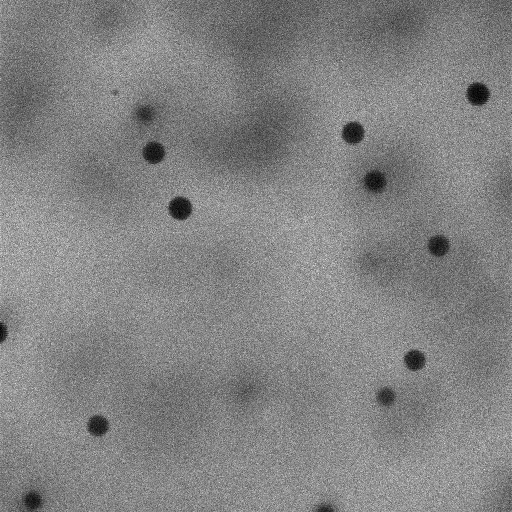
\includegraphics[width =  0.35\linewidth]{images/exp1_t41z4.png}}
\subfigure[]{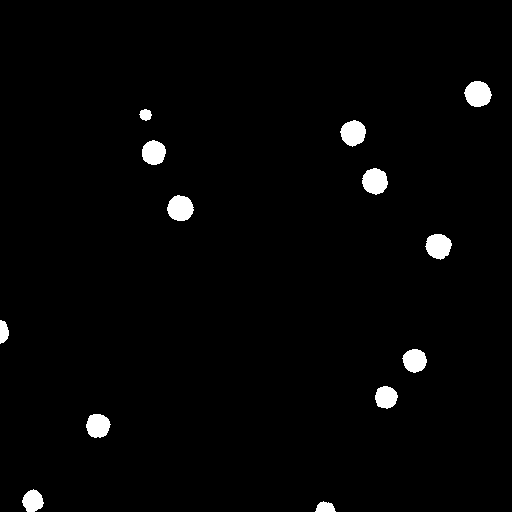
\includegraphics[width =  0.35\linewidth]{images/exp1_t41z4_bin.png}}
\subfigure[]{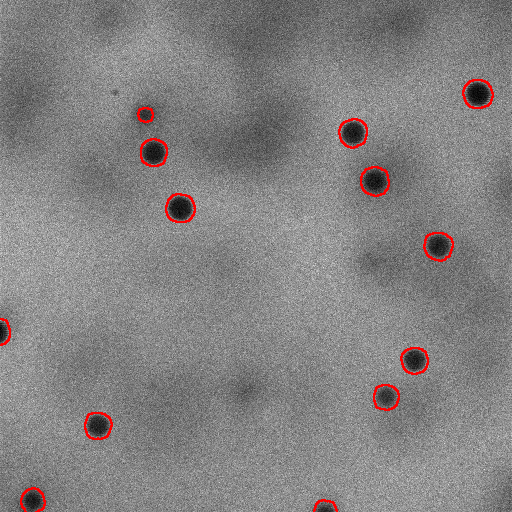
\includegraphics[width =  0.35\linewidth]{images/surimp_exp1_t41z4.png}}
\caption{Illustration of the segmentation procedure: (a) initial image, (b) result of the segmentation described in the text,  (c) overlay of the segmentation on the initial image.}
\label{fig:seg1}
\end{figure}
\vspace{1.2em}
        \item 3D regularization: 2D closing with a disk of radius 1 in the $xz$ planes.
        \item 3D individualization: beads markers are extracted using the distance transform and a watershed is applied and result is filtered using a volume criterion.
        \item Temporal identification: labels are propagated between
          two consecutive frames at $t$ and $t+1$ by finding the
          intersection between the beads at both timesteps and
          reconstructed by dilation. The remaining unlabeled beads are
          given new labels.
          \item Center bead positions are estimated separately from segmentation.
      \end{itemize}
     

%      \begin{tabular}{c@{\hskip 1em}c@{\hskip 1em}c@{\hskip 1em}c}
%        \rotatebox{90}{~~~~~~~~~~~Input} &
%        \includegraphics[trim=120 708 500 120, clip, width=.23\linewidth]{defocus2} &
%       \includegraphics[trim=120 708 500 120, clip, width=.23\linewidth]{brighter} &
%        \includegraphics[trim=120 708 500 120, clip, width=.23\linewidth]{IMG_0336_dark}\\
%        %
%        \rotatebox{90}{~~~~~~~~~Chunks} &
%        \includegraphics[width=.23\linewidth]{defocus2_chunks} &
%        \includegraphics[width=.23\linewidth]{brighter_chunks} &
%         \includegraphics[width=.23\linewidth]{IMG_0336_dark_wst}\\
%         %
%        \rotatebox{90}{~~~~~~Final decision} &
%         \includegraphics[width=.23\linewidth]{defocus2_out} &
%         \includegraphics[width=.23\linewidth]{brighter_out} &
%         \includegraphics[width=.23\linewidth]{IMG_0336_dark_out}\\
%         %
%         &
%         Defocus + flare & Noise & Low-light env \\
%      \end{tabular}
    \end{block}
    \end{column}
    %
    %\hfill
    %
    % RIGHT
    %
    \begin{column}{0.32\textwidth}
%      \begin{block}{\bf Step by step}
%
%        \vskip .5em
%
%        ~~~
%        \begin{minipage}{.154\textwidth}\centering
%          \includegraphics[width=.9\textwidth]{IMG_0336}
%          
%          Input
%        \end{minipage}
%        \hfill
%        \begin{minipage}{.154\textwidth}\centering
%          \includegraphics[width=.9\textwidth]{IMG_0336_temp_lab_filtered}
%
%          $La^{*}b^{*}$ filtered
%        \end{minipage}
%        \hfill
%        \begin{minipage}{.154\textwidth}\centering
%          \includegraphics[width=.9\textwidth]{IMG_0336_temp_grad}
%          
%          Gradient
%        \end{minipage}
%        \hfill
%        \begin{minipage}{.154\textwidth}\centering
%          \includegraphics[width=.9\textwidth]{IMG_0336_temp_wst_basins}
%          
%          Basins
%        \end{minipage}
%        \hfill
%        \begin{minipage}{.154\textwidth}\centering
%          \includegraphics[width=.9\textwidth]{IMG_0336_temp_chunks_selection_alt}
%
%          Chunks
%        \end{minipage}
%        \hfill
%        \begin{minipage}{.154\textwidth}\centering
%          \includegraphics[width=.9\textwidth]{IMG_0336_out}
%          
%          Decision
%        \end{minipage}
%        ~~~
%     \end{block}


   % ###############################################
   %\vskip .5em
    % ###############################################
    
      \begin{minipage}{1\textwidth}\centering
        \begin{block}{\bf Position estimation}
          Beads may move between
          slices due to scanning time and Brownian motion.
%      \begin{description}
        \begin{itemize}
        \item Centroid are first estimated in 2D via grey-level moments
              within labeled segmentation;
        \item Knowing the bead radius, the 3D position can be estimated by
          Pythagoras' theorem, but there is an uncertainty, since the
          center of the bead can equally well be above or below the
          considered 2D plane.
        \item The uncertainty is resolved when considering all planes
          belonging to a single bead by clustrering.
        \item In fluid media, the bead moves between plane
          acquisition, So a direct 3D centroid estimation is at best imprecise.
          \begin{figure}
            \centering
            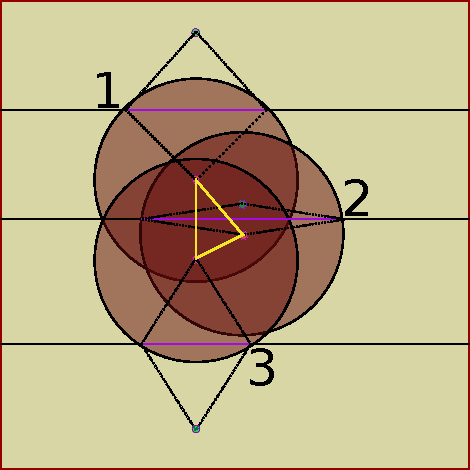
\includegraphics[width=0.71\textwidth]{images/multidepth.pdf}
            \caption{Centroid depth over multiple slice acquisition
              when the bead moves during the acquisition. Minimizing the
              perimeter of the yellow triangle characterizes the most
              likely centroid positions.}
            \label{fig:multidepth}
          \end{figure}
          
        \item Centroid estimation in 3D with imprecise bead radius can
          be achieved with a mixed Difference of Convex /
          combinatorial optimization approach described in the article.
      \end{itemize}
%        \end{description}
        \end{block}
        \end{minipage}

        %\vskip .2em
        
        % ######################################################
            \end{column}
    %
    %\hfill
    %
    % RIGHT
    %
    \begin{column}{0.32\textwidth}
        \begin{block}{\bf \color{white} Results on simulations}
          \null\centering\relax

          \newcommand{\bl}{\color{black}}
          
        \vskip -1em
        \begin{figure}
          \centering
          \subfigure[]{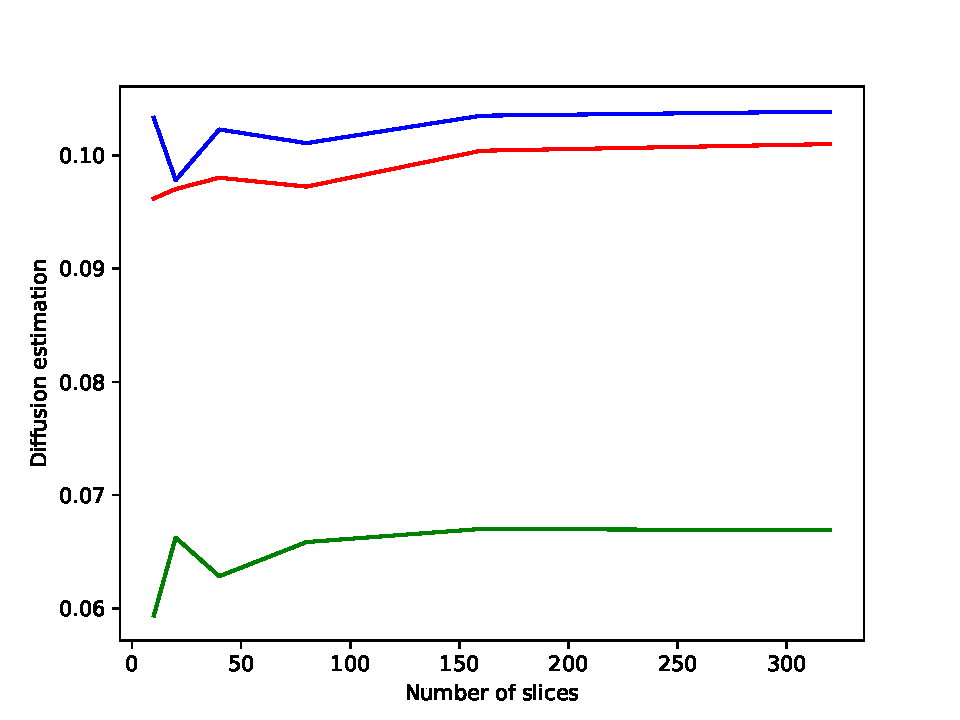
\includegraphics[width=0.45\textwidth]{images/ave_vs_smpl.pdf}}
          \subfigure[]{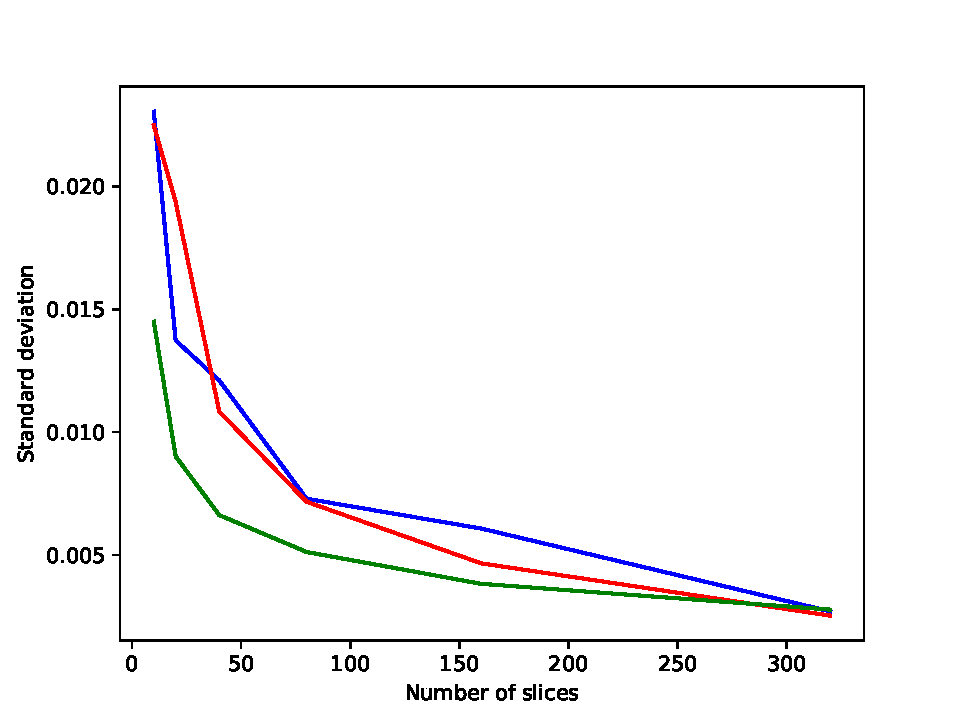
\includegraphics[width=0.45\textwidth]{images/std_vs_smpl.pdf}}
          \caption{Convergence of the diffusion estimator to a stable value (a) and its standard deviation as a function of the number of slices (b).}
        \end{figure}
        \end{block}
      %\end{minipage}
      %
      \hfill
      %
            \begin{block}{\bf \color{red} Takeaway messages}
          \null\centering\relax
        %\newcommand{\greencheck{{\color{green}\checkmark}}}

       
          %\newcommand{\bl}{\color{black}}
        \vskip -1em
        \centering
        \begin{itemize}
            \item[\cmark] Correct beads segmentation 
            \item[\cmark] Correct beads identification
            \item[\cmark] High accuracy for motion estimation (on simulated data)
            \item[\xmark] Overestimation of beads presence in z-axis;
            \item[\xmark] No ground truth for the real data diffusion coefficient.
        \end{itemize}
\begin{figure}
\centering
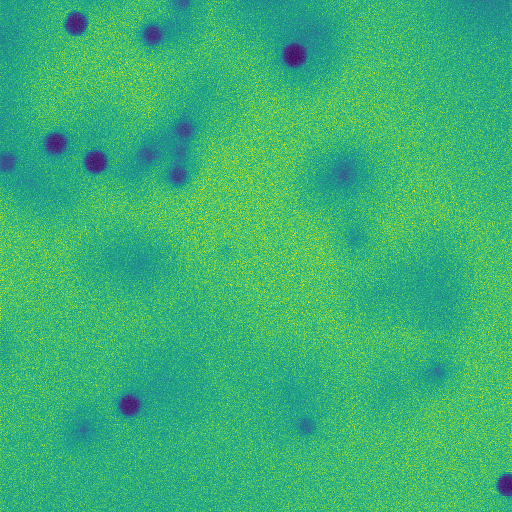
\includegraphics[width = 0.3\linewidth]{images/orig_tot.png}\hspace{0.2em}
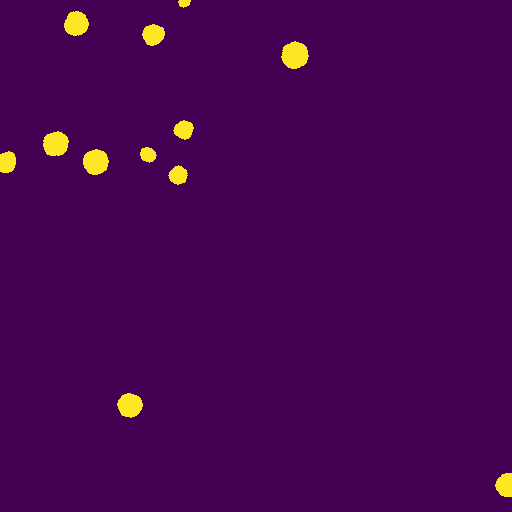
\includegraphics[width = 0.3\linewidth]{images/seg_base_tot.png}\hspace{0.2em}
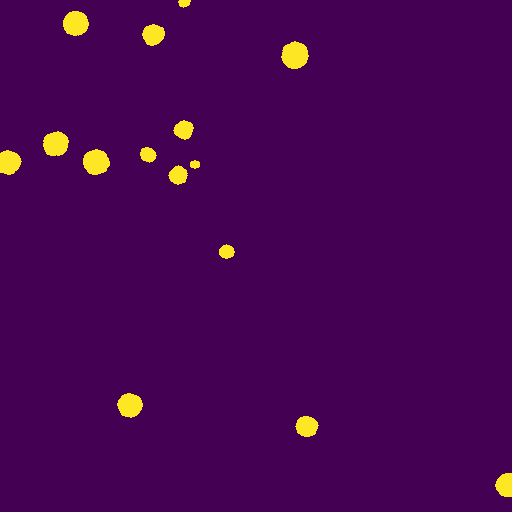
\includegraphics[width = 0.3\linewidth]{images/modif_tot.png}\\
\vspace{0.3em}
\subfigure[]{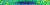
\includegraphics[width = 0.3\linewidth]{images/orig.png}}\hspace{0.2em}
\subfigure[]{
\includegraphics[width = 0.3\linewidth]{images/seg_base.png}}\hspace{0.2em}
\subfigure[]{
\includegraphics[width = 0.3\linewidth]{images/modif.png}}\\
\caption{Comparison of segmentation results: (a) original frame, (b) results of the first step of the 2D segmentation procedure before regularization, and (c) after 3D regularization. Top images are the entire $xy$ slices, and the bottom is a $xz$ view along the z-axis}
\label{fig:compa}
\end{figure}
        \end{block}
      %\begin{minipage}{.492\textwidth}\centering
%        
%        \begin{block}{\bf Some qualitative results}
%          \null\centering\color{black}
%
%        \vskip -.5em
%
%   \includegraphics[width=.17\linewidth]{IMG_0020_out} ~~
%  \includegraphics[width=.17\linewidth]{IMG_0333_out} ~~
%  \includegraphics[width=.17\linewidth]{IMG_0348_out} ~~
%  \includegraphics[width=.17\linewidth]{IMG_0341_out} ~~
%   \includegraphics[width=.17\linewidth]{IMG_0019_out}
%
%        \vskip 1em
%
%   \includegraphics[width=.17\linewidth]{IMG_0351_out} ~~
%  \includegraphics[width=.17\linewidth]{IMG_0330_out} ~~
%  \includegraphics[width=.17\linewidth]{IMG_0332_out} ~~
%   \includegraphics[width=.17\linewidth]{IMG_0346_out} ~~
%  \includegraphics[width=.17\linewidth]{IMG_0023_out}
%
%        \vskip 1em
%
%   \includegraphics[width=.17\linewidth]{IMG_0352_out} ~~
%  \includegraphics[width=.17\linewidth]{IMG_0344_out} ~~
%  \includegraphics[width=.17\linewidth]{IMG_0343_out} ~~
%  \includegraphics[width=.17\linewidth]{IMG_0334_out} ~~
%  \includegraphics[width=.17\linewidth]{IMG_0026_out}
%
%  \vskip 1em
%  
%        \end{block}
        
      %\end{minipage}
    \end{column}
    
 \end{columns}

  
% ######################################################################
% ######################################################################
% ######################################################################
  
%  \vskip .2em
    %
    %\hfill
    %
    % RIGHT
    %
    \vskip 1em
  \begin{columns}[t,totalwidth=\textwidth]
  \begin{column}{0.66\linewidth}
  \begin{exampleblock}{Conclusion}
\begin{multicols}{2}
 \begin{description}
    \item[{\bf ~~In a few words:}] ~ %
      \begin{itemize}
      \item Our method has been tested on real and simulated data;
      \item segmentation of 3D beads is performed using 2D slices;
      \item our beads tracking has a high degree of accuracy.
      \end{itemize} \bigskip %
      %

    \item[{\bf ~~Future Work:} ] ~ %
      \begin{itemize}
      \item Improve the quality and speed of our optimisation
method;
      \item Use of prior knowledge in 3D (for initial
segmentation)
      \item Release software as free and open-source
      \end{itemize}
    \end{description}
    \end{multicols}

\end{exampleblock}
  \end{column}
  
  \hfill
  \begin{column}{0.32\linewidth}
  \begin{alertblock}{\bf Selected bibliography}

 \bibliographystyle{splncs04}
\bibliography{tracking3d}
    
   % \vskip -1em
    
 %   \begin{thebibliography}{10}
  %    \newcommand{\tinysep}{\vspace*{-.1em}}

%      \renewcommand{\baselinestretch}{.98}
%      \relsize{-0.5}
  %    \centering

%      \hspace*{.1em}

    %\begin{column}{0.45\linewidth}
      
%      \tinysep
      
%    \bibitem{morpho} {\color{MyGray}{L. Najman and H. Talbot, Eds.,
 %       ``\textbf{Mathematical Morphology---From Theory to Applications},''
%        ISTE Ltd and John Wiley \& Sons Inc, 2010.}
  
 %   \end{thebibliography}
  \end{alertblock}
    \end{column}
    \end{columns}

\end{frame}

\end{document}

%%% Local Variables:
%%% mode: latex
%%% TeX-master: t
%%% ispell-local-dictionary: "american"
%%% End:
